In this section, the derivation of the plant transfer function will be investigated. To start with, we focused on the mechanical part of the system and obtained the transfer function between $X$ and $\theta$. Figure \ref{fig:mechanical_transfer} below illustrates our FBD. Further calculations are shown below. \\

\begin{figure}[H]
    \centering
    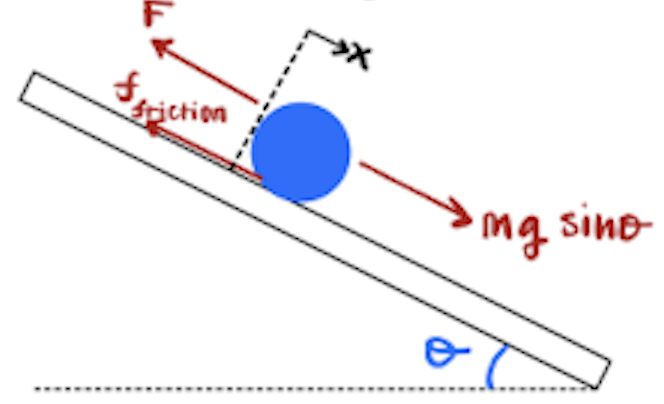
\includegraphics[width=.4\textwidth]{images/mechanical_transfer.png}
    \caption{Calculations of the first part}
    \label{fig:mechanical_transfer}
\end{figure}

\begin{gather*}
    \sum F = mg*sin(\theta) - F - f_{fric} = m\Ddot{x}\\
    sin(\theta) \approx \theta\\
    \sum F = mg*\theta - m\Ddot{x} - \mu\Dot{x} - \mu_{min}x \\
    \text{ Now, take the Laplace Transform:}\\
    m(s^2X(s)) + \mu sX(s) + \mu_{min}X(s) = mg\Theta(s)\\
    X(s)\Big(ms^2 + \mu s + \mu_{min}\Big) = mg\Theta(s)\\
    \frac{X(s)}{\Theta(s)} = \frac{mg}{ms^2 + \mu s + \mu_{min}}
\end{gather*}

Following these calculations, $\theta$ will be related to our current, $I$. After this step, two equations can be combined easily to obtain the transfer function between the current and $X$. Calculations below show the steps and derivations for these equations. 

\begin{gather*}
    i(t)*k = T = J\Ddot{\theta}\\
    I(s) * k = J*\Theta(s)* s^2\\
    \frac{\Theta(s)}{I(s)} = \frac{k}{Js^2}\\
    \text{We now combine the 2 transfer functions:}\\
    T(s) = \frac{X(s)}{I(s)} = \frac{mgk}{Jms^4 + J\mu s^3 + J\mu_{min} s^2}
\end{gather*}

Plugging in the values from the project prompt, our transfer function becomes as follows:

\begin{equation}
    T(s) = \frac{ 0.0981}{s^4 + 5 s^3 + 20 s^2}
\end{equation}